\subsection{Function - Function feature vector calculator}
\label{sec:model.function-function}
Suppose we need to compute the feature vector of $f_1$ and $f_2$ when we want to form $f_1(f_2(arg))$. $arg$ here is the argument of $f2$. The most important note is that returned type of $f_2$ must agree with one of argument types of $f_1$. The second feature is the vector of distance between the tokens mapped to two functions in the sentence. If the distance is small, they will have more chances to be composed. This is due to the usual speaking style of Vietnamese. Let us consider the following example: \\
 "{\fontencoding{T5}\selectfont con s\ocircumflex ng n\`ao ch\h{a}y qua ti\h\ecircumflex u bang missisipi?" ("what river runs through state mississippi?")}. There are at least two candidates for the result of semantic parser. They are illustrated in figure \ref{f-f.eg1} and figure \ref{f-f.eg2}. Between these two cases, our system tend to put more scores (higher value of features) on the first case. The intuition here is that, for example, "{\fontencoding{T5}\selectfont con s\ocircumflex ng}" comes before "{\fontencoding{T5}\selectfont ti\h\ecircumflex u bang}", the function $river$ is preferred to combine with $state$ to form $river(state(arg))$.
\begin{figure}[h]
\centering
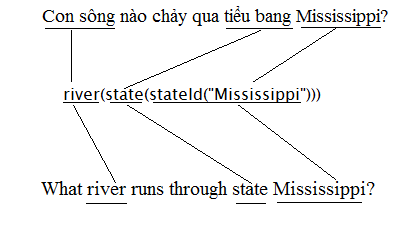
\includegraphics[scale=0.7]{eg-function-function-mapping1.png}
\caption{One result of parsing "{\fontencoding{T5}\selectfont con s\ocircumflex ng n\`ao ch\h{a}y qua ti\h\ecircumflex u bang missisipi?}"}
\label{f-f.eg1}
\end{figure}

\begin{figure}[ht!]
\centering
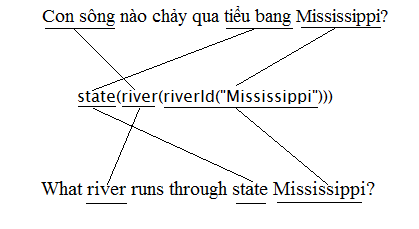
\includegraphics[scale=0.7]{eg-function-function-mapping2.png}
\caption{Another result of parsing "{\fontencoding{T5}\selectfont con s\ocircumflex ng n\`ao ch\h{a}y qua ti\h\ecircumflex u bang missisipi?}"}
\label{f-f.eg2}
\end{figure}

\subsubsection{A method of dynamic learning preference of functions compositions}
Until now, we have only one feature for describe the composition capacity of two functions. Another one is the feature which describe the compositional preferences of functions. A function is often composed with only a set some other functions. For example, $state$ function tends to receive $stateId$ function as its argument. In our approach, this feature is learned automatically through the running time of the system. 

Suppose $f1$ as a variable $p$ denoting how likely it will be composed with $f2$ to form $f1(f2(arg))$, and this composition appears in a result of semantic parser. By receiving the feedback from the outside world, we may have the answer that the result is correct or not.
\subsubsection*{If the result is correct}
In this case, we will increase the value of $p$ by formula \ref{increase-frequency}. It is clear that $p$ will be increased but it is always smaller than $M$, the maximum value of a feature.
\begin{equation}
\label{increase-frequency}
p = \frac{(p + 1)M}{M+1}
\end{equation}

\subsubsection*{If the result is wrong}
If the user says that he does not expect this answer, p needs to be decreased. Formula \ref{decrease-frequency} make the value of $p$ smaller. $p$ is also supposed to be greater or equal than $0$. 
\begin{equation}
\label{decrease-frequency}
p = \frac{p M}{M+1}
\end{equation}
\citeauthor{Clarke:2010:DSP:1870568.1870571} in \cite{Clarke:2010:DSP:1870568.1870571} also considered a feature indicating which logical symbols are usually composed together. Unfortunately, they did not clearly state the way of computing this kind of feature. If this task is done by manually configuring such feature when we define function, the result would be quite good. But that idea is not really positive with respective to scalability. Large number of functions will overwhelm annotators. 